% Energy Systems version: the 137 mm canvas of paper/figs/fig1_system.tex drawn at 119 mm (x scale 0.8686), fonts unchanged. Original: campus energy flows.
% Only the energy network is drawn: the operating periods and the capacity rules are stated in
% Sections 2.1 and 2.3 and in the caption. Canvas 137 x 80 mm; network y 3-71, legend at y 77. Coordinates in mm from
% the top-left corner, y downward. Palette: Okabe-Ito colours (electricity blue L* 46, heat vermilion L* 54, cooling
% purple L* 61).
\RequirePackage{fix-cm}
\documentclass[border=0pt]{standalone}
\usepackage[T1]{fontenc}
\usepackage{helvet}   % true point sizes (no 0.95 scaling)
\renewcommand{\familydefault}{\sfdefault}
\usepackage{amsmath}
\usepackage{sansmath}
\sansmath
\DeclareMathSizes{7.5}{8}{7}{7}   % campus mathematics: 8 pt, subscripts 7 pt
\usepackage{tikz}
\usetikzlibrary{arrows.meta,calc}
\definecolor{blue}{HTML}{0072B2}     % electricity
\definecolor{verm}{HTML}{D55E00}     % recovered heat
\definecolor{purp}{HTML}{CC79A7}     % cooling
\definecolor{slate}{HTML}{666666}    % borders
\definecolor{ink}{HTML}{222222}
\definecolor{rule}{HTML}{E6E6E6}
\definecolor{neutF}{HTML}{F5F6F7}
\definecolor{blueF}{HTML}{EAF4FA}
\definecolor{purpF}{HTML}{F8EEF4}
\newcommand{\hdg}{\fontsize{8.5}{10}\selectfont\bfseries}   % column headings
\newcommand{\cardh}{\fontsize{8}{9.5}\selectfont\bfseries}  % grid label
\newcommand{\bdy}{\fontsize{7.5}{9}\selectfont}             % body text
\newcommand{\nte}{\fontsize{7}{8.4}\selectfont}             % secondary notes
\begin{document}
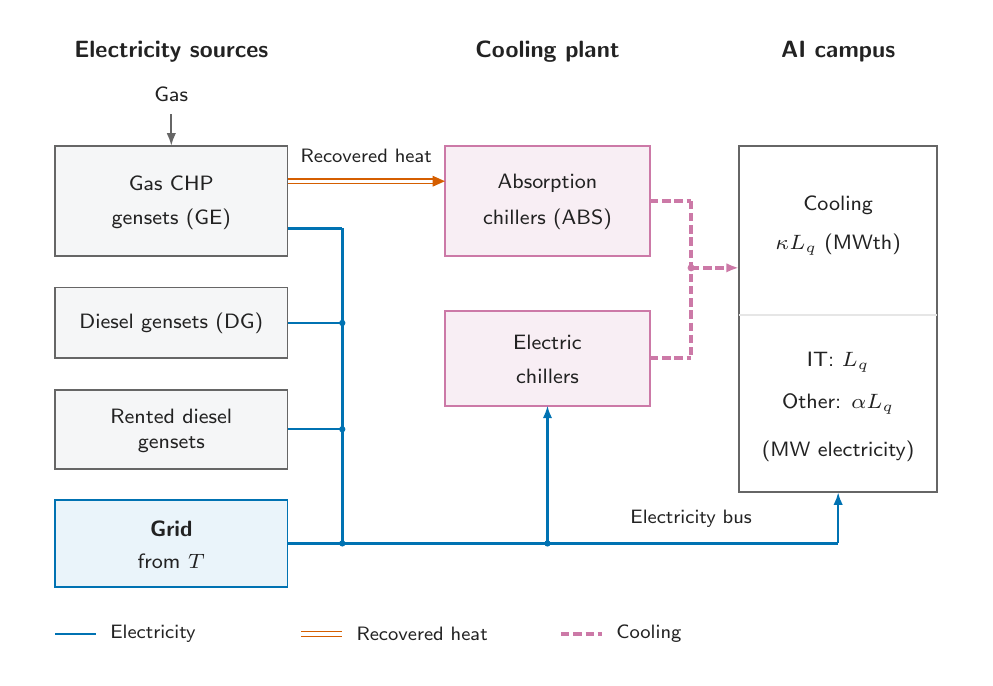
\begin{tikzpicture}[x=0.8686mm, y=-1mm, every node/.style={text=ink, inner sep=0pt},
  equip/.style={draw=slate, fill=neutF, line width=0.65pt},
  feed/.style={draw=blue, line width=0.8pt},
  bus/.style={draw=blue, line width=1.1pt},
  etip/.style={draw=blue, line width=0.8pt, -{Latex[length=1.6mm,width=1.2mm]}},
  cool/.style={draw=purp, line width=1.4pt, dash pattern=on 3pt off 1.4pt},
  ctip/.style={draw=purp, line width=1.4pt, dash pattern=on 3pt off 1.4pt, -{Latex[length=1.6mm,width=1.2mm]}}]
\path (0,0) rectangle (137,80);

\node at (21,3) {\hdg Electricity sources};
\node at (76,3) {\hdg Cooling plant};
\node at (118.5,3) {\hdg AI campus};

% supplies
\node at (21,8.5) {\bdy Gas};
\draw[draw=slate, line width=0.75pt, -{Latex[length=1.6mm,width=1.2mm]}] (21,11) -- (21,15);
\draw[equip] (4,15) rectangle (38,29);
\node at (21,19.8) {\bdy Gas CHP};
\node at (21,24.3) {\bdy gensets (GE)};
\draw[equip] (4,33) rectangle (38,42);
\node at (21,37.5) {\bdy Diesel gensets (DG)};
\draw[equip] (4,46) rectangle (38,56);
\node at (21,49.3) {\bdy Rented diesel};
\node at (21,53) {\bdy gensets};
\draw[draw=blue, fill=blueF, line width=0.65pt] (4,60) rectangle (38,71);
\node at (21,63.6) {\cardh Grid};
\node at (21,67.8) {\bdy from $T$};

% cooling plant
\draw[draw=purp, fill=purpF, line width=0.65pt] (61,15) rectangle (91,29);
\node at (76,19.8) {\bdy Absorption};
\node at (76,24.3) {\bdy chillers (ABS)};
\draw[draw=purp, fill=purpF, line width=0.65pt] (61,36) rectangle (91,48);
\node at (76,40) {\bdy Electric};
\node at (76,44.3) {\bdy chillers};

% campus
\draw[draw=slate, fill=white, line width=0.65pt] (104,15) rectangle (133,59);
\draw[draw=rule, line width=0.5pt] (104,36.5) -- (133,36.5);
\node at (118.5,22.5) {\bdy Cooling};
\node at (118.5,27.5) {\bdy $\kappa L_q$ (MWth)};
\node at (118.5,42.5) {\bdy IT: $L_q$};
\node at (118.5,47.8) {\bdy Other: $\alpha L_q$};
\node at (118.5,53.8) {\bdy (MW electricity)};

% recovered heat: GE -> ABS (double line, filled head at ABS)
\draw[draw=verm, line width=0.55pt, double=white, double distance=1.2pt] (38,19.5) -- (59.2,19.5);
\fill[verm] (59.2,18.8) -- (61,19.5) -- (59.2,20.2) -- cycle;
\node at (49.5,16.3) {\nte Recovered heat};

% electricity: feeders meet the collector without arrowheads; heads only at receiving equipment
\draw[feed] (38,25.5) -- (46,25.5);
\draw[feed] (38,37.5) -- (46,37.5);
\draw[feed] (38,51) -- (46,51);
\draw[bus] (46,25.5) -- (46,65.5);
\draw[bus] (38,65.5) -- (118.5,65.5);
\draw[etip] (76,65.5) -- (76,48);
\draw[etip] (118.5,65.5) -- (118.5,59);
\foreach \p in {(46,37.5), (46,51), (46,65.5), (76,65.5)} \fill[blue] \p circle (0.4mm);
\node at (97,62.3) {\nte Electricity bus};

% cooling: two feeders, a collector right of both chillers, one head at the campus
\draw[cool] (91,22) -- (97,22);
\draw[cool] (91,42) -- (97,42);
\draw[cool] (97,22) -- (97,42);
\draw[ctip] (97,30.5) -- (104,30.5);
\fill[purp] (97,30.5) circle (0.45mm);

% legend
\draw[draw=blue, line width=0.8pt] (4,77) -- (10,77);
\node[anchor=west] at (12,77) {\nte Electricity};
\draw[draw=verm, line width=0.55pt, double=white, double distance=1.2pt] (40,77) -- (46,77);
\node[anchor=west] at (48,77) {\nte Recovered heat};
\draw[draw=purp, line width=1.4pt, dash pattern=on 3pt off 1.4pt] (78,77) -- (84,77);
\node[anchor=west] at (86,77) {\nte Cooling};
\end{tikzpicture}
\end{document}
